\chapter{Traitement des signaux EEG}
\label{Chapitre : Traitement des signaux EEG}
\thispagestyle{fancy}

Le schéma conceptuel en annexe présente les différentes méthodes de traitement et d'analyse des signaux EEG, ainsi que les différentes interfaces cerveau-ordinateur existantes. 

\section{Caractéristiques des signaux étudiés}
\label{Section : 4.Caractéristiques des signaux étudiés}

\begin{figure}[h]
	\centering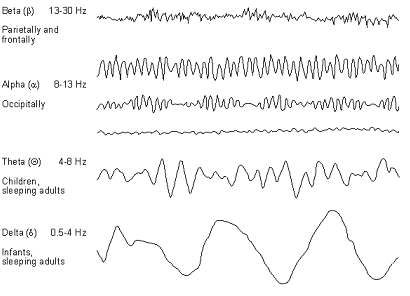
\includegraphics[width=12cm]{images/rythmesCerveau.png}
	\caption[Signaux des différents rythmes du cerveau]{Signaux des différents rythmes du cerveau.\\Source : http://www.computer.org/csdl/proceedings/bibe/2012/4357/00/06399691.pdf}
\end{figure}

A partir des rythmes du cerveau, il est possible d'extraire différentes informations, dont les 3 plus utilisées sont : 

\begin{itemize}
	\item \textbf{Information spectrale}. Variations la puissance du signal dans certaines bandes de fréquences.
	\smallbreak
	\item \textbf{Information temporelle}. Variations du signal en fonction du temps. 
	\smallbreak
	\item \textbf{Information spatiale}. Position d'une source. Pour obtenir cette information, on doit faire appel à plusieurs signaux EEG, en utilisant plusieurs électrodes.  
\end{itemize}

\section{Différentes interfaces cerveau-ordinateur}
\label{Section : 4.Différents types d'interfaces cerveau-ordinateur}

Il existe plusieurs types d'interfaces cerveau-ordinateur, les deux principales sont :
\smallbreak
\begin{itemize}
	\item Celles basées sur les activités oscillatoires. 
	\smallbreak
	\item Celles basées sur les potentiels évoqués. 
\end{itemize} 
\smallbreak
\subsubsection{Liaisons cerveau-ordinateur basées sur les activités oscillatoires}
\label{Subsection : 4.Liaisons cerveau-ordinateur basées sur les activités oscillatoires}

Il s'agit de la méthode la plus couramment utilisée. Elle consiste en l'étude des variations de la puissance sur certaines bandes de fréquence, en fonction des changements d'états mentaux de certaines zones du cerveau. Elle exploite donc l'information spatiale et spectrale. L'activité oscillatoire d'un signal EEG peut être caractérisée par deux évènements (Figure \ref{ers}):
\smallbreak 
\begin{itemize}
	\item \textbf{ERS, Synchronisation des événements liés}. Diminution de l'énergie due à l'activation corrélée du système nerveux dans certaines aires corticales.
	\smallbreak
	\item \textbf{ERD, Désynchronisation des événements liés}. Augmentation de l'énergie due à la désactivation corrélée du système nerveux dans certaines aires corticales.
\end{itemize} 
\smallbreak
Ces phénomènes oscillatoires sont essentiellement observés dans les rythmes alpha et bêta du cerveau.

\begin{figure}[h]
	\centering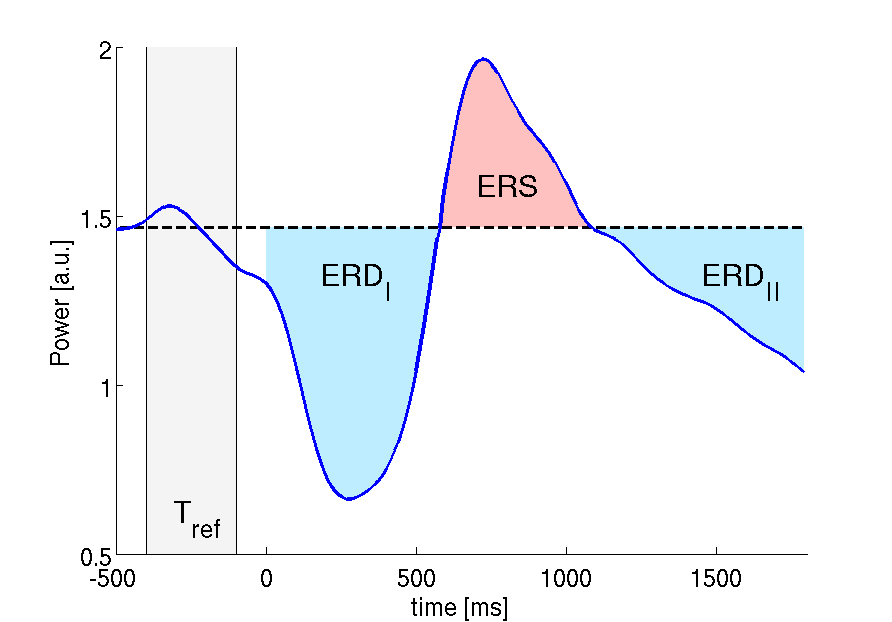
\includegraphics[width=10cm]{images/ERS_ERD.png}
	\caption[Représentation des phénomènes d'oscillations ERS et ERD du rythme bêta du cerveau]{Représentation des phénomènes d'oscillations ERS et ERD du rythme bêta du cerveau.\\Source : http://www.bbci.de/supplementary/conditionalERD/conditionalERD.htm}
	\label{ers}
\end{figure}

Les interfaces cerveau-ordinateur qui s'appuient sur les activités oscillatoires du cerveau sont principalement employées dans des dispositifs s'appuyant sur des stimulations visuelles, ou lorsqu'on fait appel à la représentation et à la visualisation mentale d'objets en mouvement. Voici les deux interfaces cerveau-ordinateur basées sur les activités oscillatoires les plus utilisées : 
\smallbreak
\begin{itemize}
	\item \textbf{SSVEP - Potentiel évoqué visuellement}. Ce dispositif repose sur une stimulation visuelle \cite{SSVEP}. En effet, lorsque la rétine est excitée par une stimulation ayant une certaine fréquence (généralement entre 3.5 Hz et 75 Hz), le cerveau génère des signaux électriques (les SSVEP) de même fréquence que le stimulus. Cette méthode a l'avantage de nécessiter une période d'entrainement relativement courte (Figure \ref{SSVEP}).
	\smallbreak
	\item \textbf{Imagerie motrice}. Ce système repose quant à lui sur des méthodes d'entrainement à l'imagination mentale, i.e. on demande à un individu de penser à une action, comme bouger un cube dans un espace en 3 dimensions \cite{motor}. On observe alors des fluctuations dans les rythmes du cerveau que l'on pourra par la suite interpréter, et en déduire l'action pensée par la personne. L'inconvénient de cette méthode est qu'elle nécessite plusieurs sessions d'entrainement. Elle n'exige cependant pas de stimulation visuelle. 
\end{itemize}
\smallbreak
\begin{figure}[h]
	\centering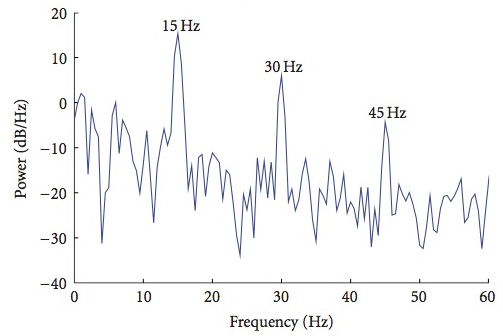
\includegraphics[width=10cm]{images/SSVEPSIgnal.jpg}
	\caption[Signal EEG de type SSVEP, en réponse à une stimulation visuelle de 15Hz]{Signal EEG de type SSVEP, en réponse à une stimulation visuelle de 15Hz.\\Source : http://www.hindawi.com/journals/cin/2010/702357/fig2/}
	\label{SSVEP}
\end{figure}

\subsubsection{Liaisons cerveau-ordinateur basées sur les potentiels évoqués}
\label{Subsection : 4.Liaisons cerveau-ordinateur basées sur les potentiels évoqués}

Il s'agit d'une méthode qui s'appuie sur l'étude  de l'information temporelle et spatiale des signaux EEG du cerveau \cite{p300}. Ce dispositif étudie les potentiels à évenements liés (ERP). Il s'agit de signaux émis par le cerveau lorsque celui-ci est excité par un stimulus (visuel, tactile, etc). Un des ERP les plus utilisé actuellement, et notamment dans le monde des jeux-vidéos est le P300. Il s'agit d'une déflexion positive qui intervient 300ms environ après la stimulation sensorielle (Figure \ref{P300}).

\begin{figure}[h]
	\centering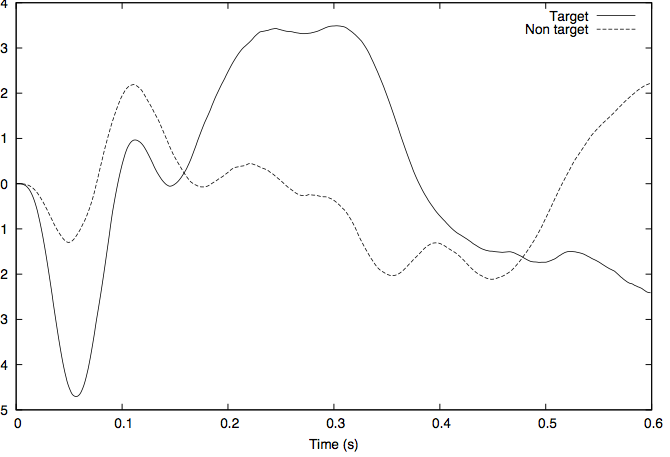
\includegraphics[width=9cm]{images/P300.png}
	\caption[Réponse P300]{Réponse P300 après un stimulus. On observe clairement la déflexion du signal après 300ms.}
	\label{P300}
\end{figure}

\section{Traitement et analyse des signaux EEG}
\label{Section : 4.Traitement et analyse des signaux EEG}

Le processus fonctionnel d'une interface cerveau-ordinateur peut être décrit comme un système en boucle fermée, composé de six étapes \cite{Saeid}\cite{Lotte} (Figure \ref{bci}) :

\begin{figure}[h]
	\centering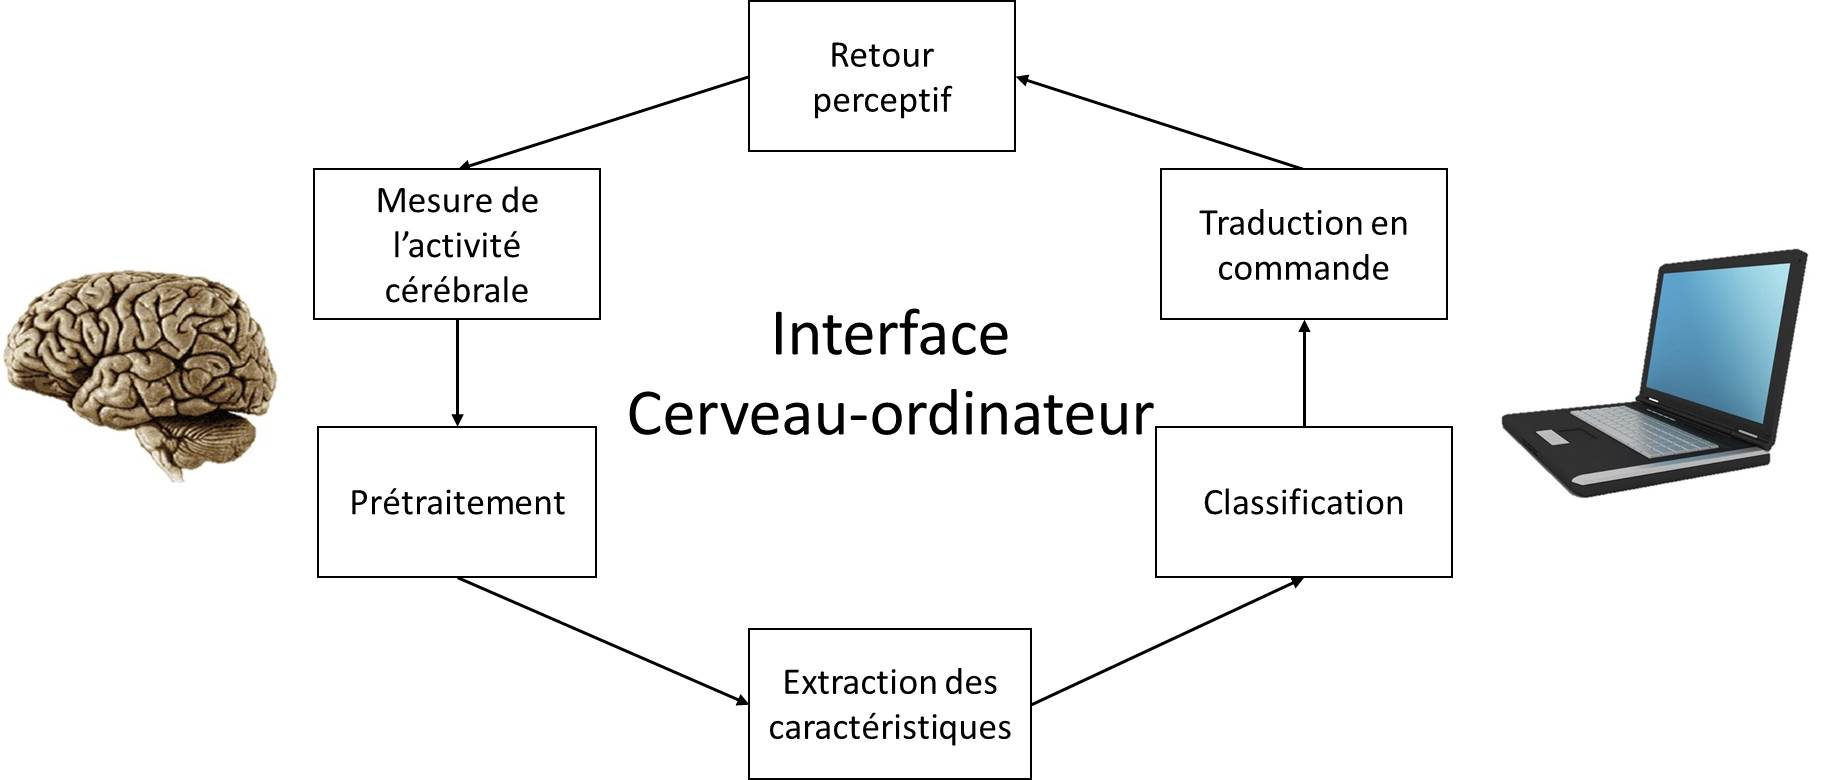
\includegraphics[width=15cm]{images/bci.jpg}
	\caption{Principales étapes constituant une interface cerveau-ordinateur.}
	\label{bci}
\end{figure}

\begin{enumerate}
	\item Mesure de l'activité cérébrale via un dispositif électroencéphalographique. On parle de phase d'acquisition des signaux. 
	\smallbreak
	\item Pré-traitement et filtrage des signaux cérébraux permettant notamment de dissocier les différents rythmes du cerveau. 
	\smallbreak
	\item Extraction des caractéristiques des signaux, afin de ne conserver que des informations pertinentes.
	\smallbreak
	\item Classification des signaux, afin d'identifier et de caractériser l'activité mentale et de l'interpréter. 
	\smallbreak
	\item Traduction en une commande envoyée à l'ordinateur. On fait ici le lien entre l'interprétation et la tâche qu'il doit effectuer.
	\smallbreak
	\item Retour perceptif. Il peut par exemple s'agir d'un retour visuel lié à l'activité neuronale perçue. L'utilisateur va ainsi progressivement apprendre à mieux contrôler le système, et ainsi boucler le synoptique de l'interface cerveau-ordinateur. 
\end{enumerate}

\smallbreak
On cherche ici a étudier le traitement et l'analyse des différents signaux EEG acquis grâce au casque EEG Emotiv. On s'intéressera principalement aux étapes 1, 2, 3 et 4. On a donc la chaîne de traitement suivante (Figure \ref{traitementEEG1}). 

\begin{figure}[h]
	\centering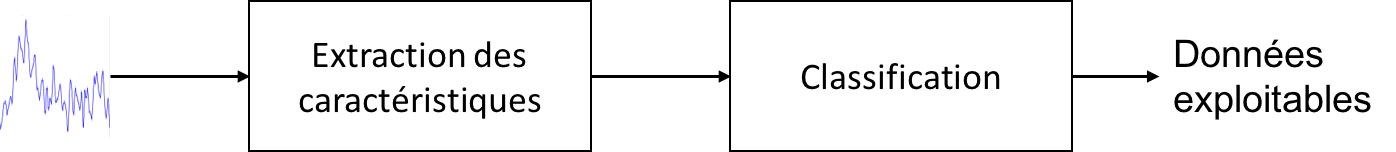
\includegraphics[width=16cm]{images/traitementEEG1.png}
	\caption{Chaine de traitement d'un signal EEG}
	\label{traitementEEG1}
\end{figure}

Cette trame est utilisée pour le traitement d'un seul signal, c'est-à-dire pour un signal provenant d'une seule électrode. Or, étudier le signal de plusieurs électrodes permet d'augmenter la précision du système. Cela permet également d'accéder à une information supplémentaire : la localisation spatiale des signaux. Ce type de procédé augmente inévitablement la quantité de calculs à effectuer, d'autant plus que les informations doivent être traitées en temps réel. Pour palier à ce problème, on ajoute une étape d'optimisation des données (prétraitement) afin de réduire le nombre d'informations à manipuler. On obtient donc cette nouvelle chaine de traitement (Figure \ref{traitementEEG2}) : 

\begin{figure}[h]
	\centering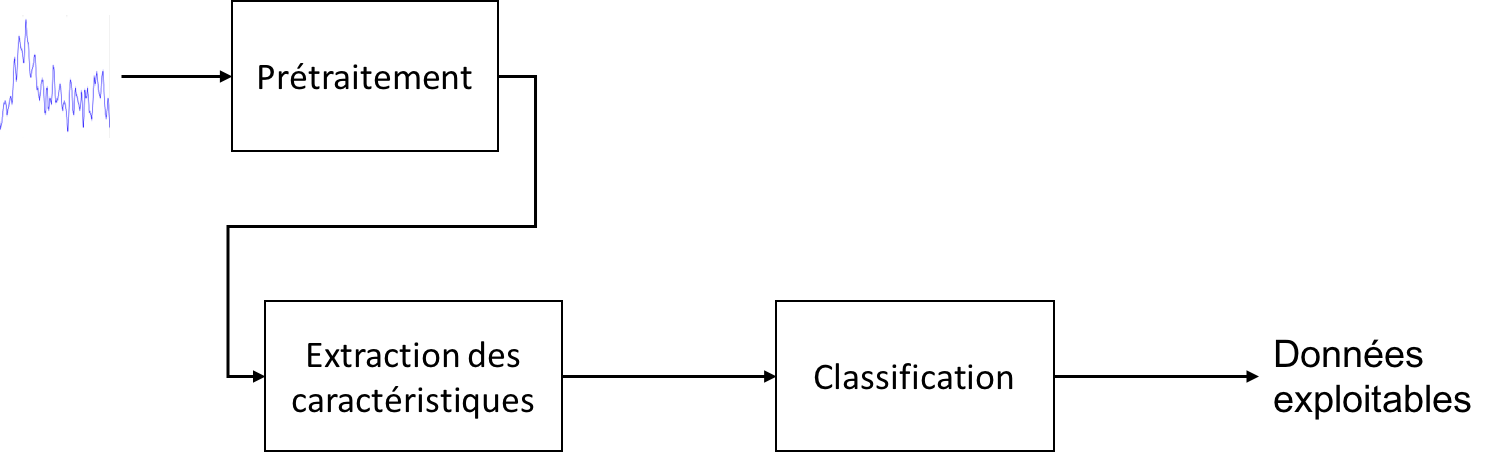
\includegraphics[width=14cm]{images/traitementEEG2.png}
	\caption{Chaine de traitement de plusieurs signaux EEG}
	\label{traitementEEG2}
\end{figure}

\subsection{Pré-traitement, méthodes d'optimisation des données}
\label{Subsecton : 4.Pré-traitement, méthodes d'optimisation des données}

Il existe différents algorithmes d'optimisation des données, afin de réduire la quantité d'informations à traiter en temps-réel \cite{Lotte}.
\smallbreak
\begin{itemize}
	\item \textbf{Sélection des caractéristiques.} Algorithme permettant de sélectionner automatiquement les données les plus pertinentes. 
	\smallbreak
	\item \textbf{Sélection des entrées (électrodes).} Sélectionne automatiquement les électrodes dont les données sont les plus pertinentes. Cet algorithme est en général plus efficace que les méthodes de sélection des caractéristiques.
	\smallbreak 
	\item \textbf{Filtrage spatial.} On réalise une combinaison lineaire des signaux issus des électrodes par suppression des redondances afin de réduire la quantité d'informations à traiter. 
\end{itemize}

\subsubsection{Filtrage spatial}
\label{Subsubsecton : 4.Filtrage spatial}
Le filtrage spatial permet de réduire la quantité d'informations à traiter en fusionnant des chaines entres elles \cite{Lotte} \cite{Saeid} . Il a également un sens du point de vu physiologique car il permet de retrouver les signaux sources. On définit donc le filtrage spatial comme une combinaison linéaire de l'ensemble des chaines, chaque chaine étant pondérée par un poids : 

\begin{equation}
		\tilde{x}=\sum{w_i*x_i}
\end{equation}

Où $\tilde{x}$ est le signal filtré spatialement, $i$ le canal traité, $w_i$ le poids attribué à $i$, $x_i$ le signal EEG de $i$.

Il existe plusieurs méthodes de filtrage spatial : 
\smallbreak
\begin{itemize}
	\item  \textbf{Filtrage spatial fixe.} Dans un filtrage fixe, le poids attribué à chaque canal est prédéterminé par l'utilisateur. On utilise cette méthode principalement pour réduire le bruit de fond. En voici deux couramment utilisées : 
	\smallbreak
	\subitem \textbf{Filtre Bipolaire.} On calcule la différence entre deux canaux à proximité du canal que l'on souhaite étudier : $ C_z = FC_3 - C_4 $, où $C_z$, $FC_3$ et $C_4$ correspondent au placement des électrodes selon la norme Internationale 10-20.
	\smallbreak
	\subitem \textbf{Filtre Laplacien.} $ C_z = 4C_z-F_z-P_z-C_3-C_4$. où $C_z$, $F_z$,$P_z$,$C_3$, et $C_4$ correspondent au placement des électrodes selon la norme Internationale 10-20.
	\smallbreak
	\item \textbf{Filtrage spatial avec apprentissage.} Les poids sont déterminés automatiquement, grâce à un d'apprentissage.
	\smallbreak
	\subitem\textbf{PCA, Analyse en composantes principales.} La PCA permet d'extraire des informations à partir de signaux bruités et de réduire le nombre de données à traiter.
	\smallbreak
	\subitem\textbf{ICA, Analyse en composantes indépendantes.} L'ICA est utilisée en BSS (Séparation des sources masquées), c'est-à-dire lors de l'extraction de sources à partir de plusieurs signaux (ex: identifier et extraire une voix dans une soirée à partir de plusieurs microphones).
	\smallbreak 
\end{itemize}

On s'intéressera ici plus particulièrement aux filtres spatiaux avec apprentissage car la sélection des poids à appliquer à chaque chaine est faite automatiquement.

\subsubsection{Analyse en composantes principales (PCA)}
\label{Subsubsecton : 4.PCA}
 C'est une méthode d'analyse statistique des données qui permet d'extraire certaines informations à partir d'un flot de données diffus. On réduit ainsi la complexité des données. Pour cela, on les exprime dans un nouveau repère en effectuant une transformation linéaire, afin de décorréler les données entres elles. Un flot de donnée peut être caractérisé par deux informations : le bruit et la redondance \cite{Lotte}.
 
 Soit $X$ une matrices contenant les échantillons de données de plusieurs sources ($m$x$n$, $m$ correspondant aux différentes sources $X_i$ avec $0<i<m$, $n$ aux valeurs des sources à chaque instant $t$ avec $0<j<n$), $Y$ la ré-écriture de $X$ dans le nouveau repère. On cherche donc à déterminer la transformation linéaire $P$ permettant de réduire à la fois le bruit et la redondance des données  \cite{PCA}, tel que 
 \begin{equation}
 	 Y = PX
 \end{equation}

 Avec :
   
   \begin{equation}
   \begin{blockarray}{cccccc}
   & t_1 & t_2 & t_3 & ... & t_{fin} \\
   \begin{block}{c(ccccc)}
   X_1 &  &  &  &  &  &  \\
   X_2 &  &  &  &  &  &  \\
   X_3 &  &  &  &  &  &  \\
   ... &  &  &  &  &  &  \\
   X_m &  &  &  &  &  &  \\
   \end{block}
   \end{blockarray} = X
    \end{equation}
 
\paragraph{Le bruit.} Il est exprimé par l'équation $SNR = \frac{\sigma^2_{signal}}{\sigma^2_{bruit}}$, avec $SNR$ (Signal Noise Ratio) la mesure du bruit, $\sigma^2_{signal}$ la variance du signal et $\sigma^2_{bruit}$ la variance du bruit. Plus la valeur SNR est élevée, plus le signal est pur (sans bruit)  \cite{PCA}  \cite{PCA2}. La variance caractérisant la dispersion d'un jeu de donnée autour de sa moyenne, on cherche donc à déterminer la transformation linéaire qui la maximise (Figure : \ref{bruit_PCA}).

\begin{figure}[h]
	\centering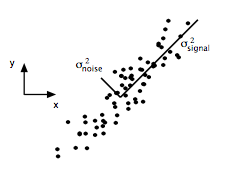
\includegraphics[width=8cm]{images/PCA_donnees.png}
	\caption[Bruit du flux de donnée $X$ et $Y$.]{Flux de données e $X$ et $Y$. On représente ici la variance du bruit ainsi que du signal. \cite{PCA}}
	\label{bruit_PCA}
\end{figure}

\paragraph{La redondance des données.} Plusieurs électrodes peuvent avoir enregistré la même information \cite{PCA}  \cite{PCA2}. On cherche donc à supprimer ses informations répétitives afin de diminuer la quantité d'informations à traiter. La mesure de la covariance représentant le degrés de relation linaire entre deux jeux de données. On recherche alors la transformation linéaire permettant de diminuer sa valeur (figure : \ref{redondance}).   

\begin{figure}[h]
	\centering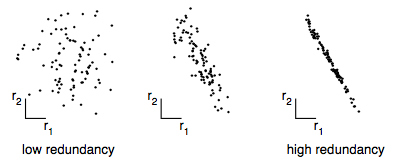
\includegraphics[width=12cm]{images/redondance.png}
	\caption[Redondances possibles dans les données dans deux flux de données R1 et R2.]{Redondances possibles des données dans deux flux de données R1 et R2. Les deux mesures à gauche ne sont pas corrélées. Les deux mesures à droite sont quant à elles fortement corrélées. \cite{PCA}}
	\label{redondance}
\end{figure}

\paragraph{La matrice de covariance.} Elle est constituée de la covariance et de la variance d'un ensemble de jeux de données \cite{PCA2}. On cherche donc à maximiser la variance (donc SNR) et à annuler les valeurs de covariances (i.e. réduire la redondance). La solution optimale revient donc à diagonaliser la matrice.

\[M =\begin{bmatrix}
\sigma^2_{x_1} & \sigma_{x_1x_2} & ... &\sigma_{x_1x_m}
\\\sigma_{x_2x_1} & \sigma^2_{x_2} & ... &\sigma_{x_2x_m} 
\\ ...&... &\sigma^2_{x_3} &...
\\ \sigma_{x_mx_1}&\sigma_{x_mx_2} & ...&\sigma^2_{x_m}  
\end{bmatrix}\]

\paragraph{Diagonalisation de la matrice de covariance.} Soit $S_X$ la matrice de covariance de $X$, on cherche à déterminer la transformation linéaire $P$, de manière à ce que $S_Y$, la matrice de covariance de $Y$, soit diagonalisée \cite{PCA}  \cite{PCA2}. 
On a donc : 
\begin{equation}
	\begin{split}
	 S_Y &= \frac{1}{n}YY^T \\
	&= \frac{1}{n}(PX)(PX)^T \\
	&= \frac{1}{n}PXX^TP^T \\
	S_Y &= PS_XP^T 
	\end{split}
\end{equation}
D'après le théorème de diagonalisation orthogonale d'une matrice symétrique (une matrice de covariance étant par définition symétrique), $S_X$ peut être exprimée par $EDE^T$, où $D$ est une matrice diagonale et $E$ est la matrice de vecteurs propres de $A$, arrangés en colonnes. On sélectionne $P$ de manière à ce que chacune de ses colonnes soit un vecteur propre de $S_X$. On pose  $P = E^T$, on a donc $ A = P^TDP$.

On obtient : 
\begin{equation}
	\begin{split}
	S_Y &= PS_xP^T \\
	& = P(E^TDE)P^T \\
	& = P(P^TDP)P^T \\
	& = (PP^T)D(PP^T) \\
	& = (PP^{-1})D(PP^{-1})\\
	S_Y& = D\\ 
	\end{split}
\end{equation}

Le choix de $P$ diagonalise bien $S_X$. Les composantes principales de $X$ sont les vecteurs propres de $S_X$.

\paragraph{Algorithme du PCA} \cite{PCA}  \cite{PCA2}:
\begin{enumerate}
	\item Soustraire la moyenne de chaque source à elle même. La moyenne des données devient alors nulle, simplifiant ainsi le calcul de la variance et de la covariance.
	\item Calculer la matrice de covariance. 
	\item Calculer les valeurs propres et vecteurs propres de la matrice de covariance. 
	\item Trier les vecteurs propres en fonction de la valeur des valeurs propres qui y sont rattachées (du plus grand au plus petit). Le vecteur des valeurs propres triées correspond au vecteur caractéristique. 
	\item Dériver les nouvelles données. On multiplie la transposée du vecteur caractéristique par les données dé-moyennées.   
\end{enumerate}

\subsubsection{Analyse en composantes indépendantes (ICA)}
\label{Subsecton : 4.ICA}
La méthode de filtrage spatiale par analyse des composantes indépendantes permet de réduire le nombre de données à traiter comme la PCA. De plus, elle permet de retrouver les signaux sources à partir des signaux enregistrés par les électrodes\cite{ICA} (Figure : \ref{conceptBSS}). 

\begin{figure}[h]
	\centering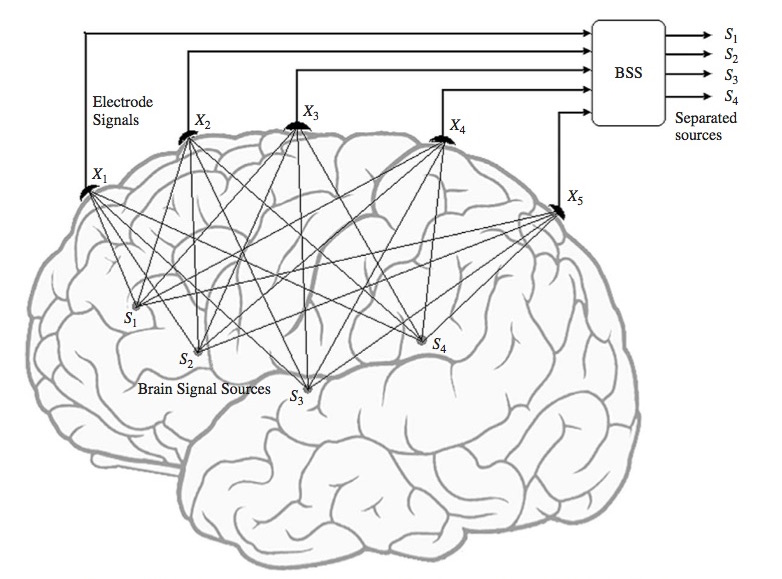
\includegraphics[width=0.6\textwidth]{images/conceptBSS.jpg}
	\caption[ICA et principe du BSS]{Principe du BSS appliqué à la détection de sources des caractéristiques du cerveau humain. $Si$ correspondent aux sources et $xi$ aux électrodes mesurant les signaux à la surface du crâne.\cite{Saeid}}
	\label{conceptBSS}
\end{figure}

Soient $S_i$ les signaux sources indépendants (l'amplitude de $S_1$ ne dépend pas de celle de $S_2$), $X_i$ les signaux enregistrés par les électrodes, $A$ la transformation linéaire mixant les sources $S_i$ en $X_i$.

\begin{equation}
X_i = AS_i
\end{equation}

 Le but est donc de retrouver la matrice $A$ et son inverse afin de reconstruire les signaux sources $S_i$ à partir de ceux observés $X_i$. Soit $S_i'$ une estimation des sources $S_i$, on doit donc déterminer la matrice $W$, elle même une approximation de $A^{-1}$

 \begin{equation}
 S_i' = WX_i
 \end{equation}

On a alors une équation à deux inconnues, ce qui est impossible à résoudre sous la forme actuelle. Une solution est d'utiliser la décomposition en valeurs singulières (SVD). 

\paragraph{La décomposition en valeurs singulières.} Une matrice est décomposable en trois opérations linéaires simples \cite{ICA}:
\smallbreak
\begin{itemize}
	\item Une rotation $V$. Il s'agit alors d'une matrice orthogonale. 
	\smallbreak
	\item Un étirement (ou compression) $\Sigma$. Il s'agit alors d'une matrice diagonale. 
	\smallbreak
	\item Une rotation $U$. Il s'agit alors d'une matrice orthogonale. 
\end{itemize}

tel que : 
\begin{equation}
	A = U\Sigma V^T
\end{equation}

Avec $A \in R^{m\times n}$, $U \in R^{m\times m}$,$\Sigma \in R^{m\times n}$,$ V \in R^{n\times n}$.

Cette transformation linéaire s'apparente à un changement de repère, ce qui n'est pas sans rappeler la méthode utilisée pour la PCA (Figure : \ref{svd}). 

\begin{figure}[h]
	\centering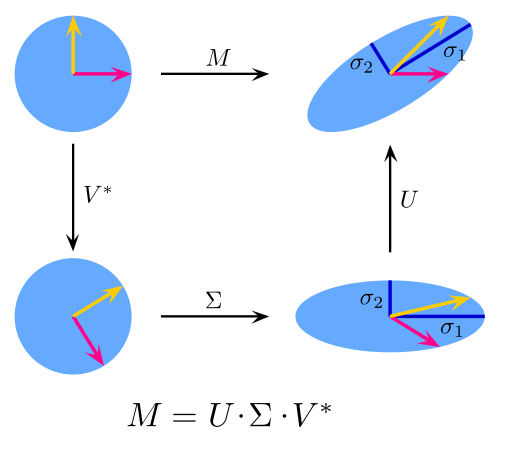
\includegraphics[width=0.6\textwidth]{images/SVD.png}
	\caption[Décomposition en valeurs singulières]{La décomposition en valeurs singulières s'apparente à décomposer une matrice en trois opérations linéaires simples : deux rotations $U$ et $V$ et un étirement $\Sigma$. $\sigma_1$ et $\sigma_2$ correspondent aux valeurs singulières. \\Source : https://fr.wikipedia.org/wiki/Décomposition\_en\_valeurs\_singulières}
	\label{svd}
\end{figure}

On peut écrire : 
\begin{equation}
	W = A^{-1} = V \Sigma^{^-1} U^T
\end{equation}

\paragraph{Étude de la covariance de $X_i$.}
On émet l'hypothèse suivante : soit $S_X$ la covariance des signaux sources, on a $S_X = I$ (une matrice de covariance étant par définition symétrique). De plus, on rappelle que pour une matrice orthogonale, $V^{-1}=V^T$. La covariance des signaux observés par les électrodes peut alors être exprimée comme suit : 
\begin{equation}
\begin{split}
S_X &= \frac{1}{n}XX^T \\
&= \frac{1}{n}(AS)(AS)^T \\
& = \frac{1}{n}(U\Sigma V^TS)(U\Sigma V^TS)^T  \\
& = U\Sigma V^T(\frac{1}{n}SS^T)V\Sigma U^T  \\
& = U\Sigma V^{-1}V\Sigma U^T \\
S_X &=  U\Sigma^2 U^T \\
\end{split}
\end{equation}

Si on pose $E = U$ avec $E$ une matrice dont les colonnes correspondent aux vecteurs propres de $S_X$, $D = \Sigma^2$ avec $D$ une matrice diagonale. On obtient alors :
\begin{equation}
	S_X = EDE^T
\end{equation}

Ce qui correspond à la propriété sur les matrices symétriques qui dit qu'une matrice peut être diagonalisée par ses vecteurs propres. 
On peut alors reformuler la valeur de $W$ : 
\begin{equation}
	W = VD^{-\frac{1}{2}}E^T
\end{equation}

Multiplier par $D^{-\frac{1}{2}}E^T$ revient jusqu'ici à réaliser une analyse en composantes principales, c'est à dire à supprimer les composantes dépendantes (redondance des informations). Soit $X_w = D^{-\frac{1}{2}}E^TX$ les données de $X$ dont les dépendances ont été supprimées et d'après l'équation 4.4, on a :
\begin{equation}
	S_i' = VX_w
\end{equation}

Il nous reste donc à caractériser la transformation linéaire $V$.
 
\paragraph{Résolution de V.} On cherche la valeur de la matrice de rotation $V$ tel que les sources $S_i'$ soient statistiquement indépendantes \cite{ICA}. i.e. 

\begin{equation}
	P(s) = \prod P(S_i)
\end{equation}

Avec P(s) la loi de probabilité de la source $S$ et $P(S_i)$ la loi de probabilité de l'ensemble des sources $S_i$.
La mesure des statistiques indépendantes entre plusieurs variables peut être déterminée par l'équation de multi-information suivante :

\begin{equation}
	I(S) = \int{P(S)log_2 \frac{P(S)}{\prod_iP(S_i)}dy}
\end{equation}

Si $I(S) = 0$, cela signifie que les sources sont totalement indépendantes. En effet, si $P(S) = \prod_i P(S_i)$, on a $log(\frac{P(S)}{\prod_iP(S_i)}) = log(1) = 0$. Il faut donc trouver la matrice $V$ tel que $I(S) = 0$.

\paragraph{Algorithme de l'ICA} \cite{ICA}
\smallbreak
\begin{enumerate}
	\item Soustraire la moyenne de chaque source à elle même. La moyenne des données devient alors nulle, simplifiant ainsi le calcul de la variance et de la covariance.
	\item Calculer la matrice de covariance. 
	\item Calculer les valeurs propres $D$ et vecteurs propres $E$ de la matrice de covariance.
	\item Dériver les nouvelles données. On multiplie la transposée du vecteur caractéristique par les données dé-moyennées. Le résultat correspond aux signaux observés sur les électrodes, dont on a supprimé les dépendances. Soit $E^TX$.
	\item Multiplier le résultat précédent par la racine du vecteur des valeurs propres. soit $X_w = D^{-\frac{1}{2}}E^TX$.
	\item Calculer la rotation ($V$) qui maximise la corrélation des données. 
	\item Calculer $W = VD^{-\frac{1}{2}}E^T$.
	\item On peut alors retrouver les signaux sources $S_i$ en calculant $S_i = W \times X_0$.
\end{enumerate}

Les étapes 1 à 4 correspondent à une analyse en composantes principales.

\subsubsection{Configuration Spatiale Commune (CSP)}
\label{Subsubsecton : 4.CSP}
La méthode CSP est utilisée à la fois en filtrage spatial et pour les algorithmes de sélection automatique de canaux (signaux de sortie des électrodes) \cite{CSP} \cite{Lotte}. Tout comme l'algorithme du PCA, on cherche ici à réaliser une transformation linéaire sur un flot de données, afin de décorréler les sources entres elles. À la différence qu'ici, on a en entrée du filtre deux jeux de données, que l'on appellera des classes. Dans notre cas, il peut s'agir d'une classe "stimulus gauche" correspondant aux signaux générés après le mouvement de la main gauche, ou d'une classe "stimulus droit" correspondant aux signaux générés après le mouvement de la main droite. On cherche alors à maximiser la variance et à minimiser la covariance entre les deux classes. On a donc deux étapes principales : 
\smallbreak
\begin{enumerate}
	\item Maximiser la variance et minimiser la covariance des sources de chacune des classes. 
	\smallbreak
	\item Maximiser la variance de chacune des deux classes et minimiser la covariance entre les deux classes.  
\end{enumerate}

Soit $R_H$ et $R_F$ les covariances des classes $H$ et $F$, tels que :

\begin{equation}
	R_H = \frac{X_H X^T_H}{Trace(X_H X^T_H)} \ \ R_F = \frac{X_F X^T_F}{Trace(X_F X^T_F)}
\end{equation}

Avec $X_H$ et $X_F$ les données de la classe $H$ et $X_F$ les données de la classe $F$. 
La covariance spatiale totale correspond à la somme des covariances des deux classes : 

\begin{equation}
	R = R_H + R_F 
\end{equation}

\paragraph{Algorithme du CSP}
\begin{enumerate}
	\item Soit $X_g$ un ensemble de sources de données EEG  correspondant aux réponses cérébrales lors du mouvement de la main gauche et $X_d$ un ensemble de données correspondant aux réponses cérébrales lors du mouvement de la main droite. On soustrait la moyenne de chacune des sources des deux ensembles à elles-mêmes. La moyenne des données devient alors nulle, simplifiant ainsi le calcul de la variance et de la covariance.
	\item Calculer la matrice de covariance des deux ensembles $X_g$ et $X_d$. On appellera $R_g$ la matrice de covariance de l'ensemble $X_g$ et $R_d$ la matrice de covariance de l'ensemble $X_d$.
	\item Calculer les valeurs propres $D$ et vecteurs propres $E$ de la matrice de $R_g$ et $R_d$.
	\item Dériver les nouvelles données. On multiplie la transposée du vecteur caractéristique par les données dé-moyennées. Le résultat correspond aux signaux observés sur les électrodes, dont on a supprimé les dépendances, soit $E^TX$.
	\item Multiplier le résultat précédent par la racine du vecteur des valeurs propres. soit $X_w = D^{-\frac{1}{2}}E^TX$.
	\item Calculer la valeur des sources des deux ensembles, soit $S_g = WR_gW^T$ et $S_d = WR_dW^T$.
	\item Calculer la rotation ($V$) qui maximise la corrélation des données. 
	\item Calculer $W = VD^{-\frac{1}{2}}E^T$.
	\item Calculer les valeurs propres $D$ et vecteurs propres généralisés $B$ des sources $S_g$ et $S_d$.
	\item Trier les vecteurs propres en fonction de la valeur des valeurs propres qui y sont rattachées (du plus grand au plus petit).
	\item Le calcul du poids à attribuer à chacun des canaux est déterminé de la manière suivante : $Poids = B'W$
\end{enumerate}


\subsection{Méthodes d'extraction des caractéristiques}
\label{Subsecton : 4.Méthodes d'extraction des caractéristiques}

\subsubsection{Filtrage temporel}
\label{Subsub : 4.Méthodes d'extraction des caractéristiques}
La phase d'extraction des données consiste dans un premier temps à réaliser un filtrage temporel afin d'extraire du signal EEG les rythmes du cerveau (caractéristiques) qui nous intéressent. Pour cela, on réalise un filtrage passe-bande. Les deux types de filtres les plus utilisés en traitement du signal sont les filtres de Butterworth et Chebychev. 

\begin{itemize}
	\item \textbf{Filtre de Butterworth.} Il s'agit d'un filtre qui possède un gain quasiment constant dans sa bande-passante (on parle de critère de méplat). L'avantage est qu'il engendre très peu de distorsions dans la bande passante. Sa réponse en phase est presque linéaire. Cependant sa réjection est moins importante dans la bande coupante, dû à la "limitation" de la bande de coupure.
	\smallbreak
	\item \textbf{Filtre de Chebychev.} Il s'agit d'un filtre dans lequel on introduit une oscillation (distorsion contrôlée), permettant d'obtenir une "vitesse" de coupure plus importante. L'inconvénient de ce filtre est que les oscillations introduites entrainent des distorsions de phase sur le signal de sortie. 
	\smallbreak
\end{itemize}

Il est préférable d'utiliser une filtre de type Butterworth dans notre cas car on ne peut pas tolérer l'introduction de distorsions dans les rythmes du cerveau. On propose donc d'utiliser un filtre passe-bande d'ordre 5.

\subsubsection{Représentation spectrale}

Une fois les caractéristiques extraites, on souhaite les représenter dans le domaine spectral afin de structurer les données pour la classification. La méthode majoritairement utilisée dans le traitement des signaux EEG est la transformée de Fourier à court terme (TFCT). Il s'agit d'une méthode dérivée de la transformée de Fourier rapide (FFT) qui gère la non-stationnarité des signaux d'entrée en les fenêtrant. Concrètement, cela revient à calculer la FFT, puis à appliquer un fenêtrage \cite{feature}.
 
 \begin{center}
 $
 STFT(x(t)) = X(\tau,u) = \int_{-\infty}^{\infty}x(t)w(t-\tau)e^{-j2\pi.ut}dt
 $
\end{center}

Avec $X(t,\tau)$ la transformée de $x(t)w(t-\tau)$, $x(t)$ le signal à transformer, $w(t)$ le signal de fenêtrage, $\tau$ la valeur de décalage temporel des fenêtres et $u$ la fréquence. Il s'agit la plupart du temps d'un fenêtrage de pondération de Hanning ou de Gauss, qui offre à la fois une bonne résolution spectrale et une bonne dynamique au filtrage. 
Si on discrétise les valeurs, on obtient le calcul de la STFT suivant : 

 \begin{center}
$
 STFT(x[n])=\sum_{0}^{N-1}x(n)w(n-m)e^{-j2.\pi\frac{nk}{N}}
 $
 \end{center}
 
 avec $k$ l'échantillon calculé, $N$ le nombre de points et $n$ la variable.
 
 La largeur des fenêtres étant constante, on observe une diminution de la résolution temporelle lorsque les fréquences deviennent trop faibles.

\begin{figure}[h]
	\centering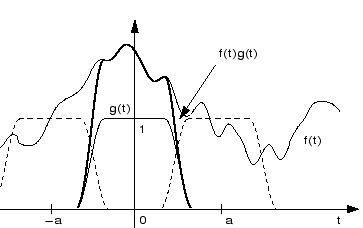
\includegraphics[width=9cm]{images/STFT.png}
	\caption[STFT du signal f(t), avec fenêtrage par le signal g(t)]{STFT du signal f(t), avec fenêtrage par le signal g(t)\\https://www.math.ucdavis.edu/~strohmer/research/gabor/gaborintro/img47.gif}
	\label{stft}
\end{figure}

\subsection{Méthodes de classification}
\label{subsection : 4.Méthodes de classification}
La phase de classification consiste à trier et à classifier des échantillons dans une catégorie (classe). 

Dans le cas général, les données d'entrées sont les suivantes :
\smallbreak
\begin{itemize}
	\item P classes d'objets du même type.
	\smallbreak
	\item N observables définies pour toutes les classes.
	\smallbreak
	\item Pour chacun des P classes, un échantillon d'objets Nk  (k étant l'indice de classe).
	\smallbreak
\end{itemize}

Pour classifier un nouvel objet dans une des classes définies, on passe par cinq phases distinctes :
\smallbreak
\begin{itemize}
	\item La collecte des données.
	\smallbreak
	\item La caractérisation des classes.
	\smallbreak
	\item Le choix d'un algorithme de classification.
	\smallbreak
	\item L'apprentissage.
	\smallbreak
	\item Les tests.
	\smallbreak
\end{itemize}

Nous avons étudié les 3 algorithmes de classification suivants et nous les avons comparé en fonction leurs applications possibles, leurs avantages et leurs inconvénients \cite{Faivre}.

\subsubsection{Linear Discriminant Analysis}
\label{Subsubsection : 4.Linear Discriminant Analysis}
L'analyse discriminante linéaire (LDA) est l'algorithme le plus populaire dans le domaine des interfaces cerveau-ordinateur (BCI).

Il est réputé comme étant un classificateur stable en raison de sa faible complexité, il s'appuie sur des calculs simples, et est adapté à la classification en temps réel (Figure \ref*{classiLDA}).
 
\begin{figure}[h]
	\centering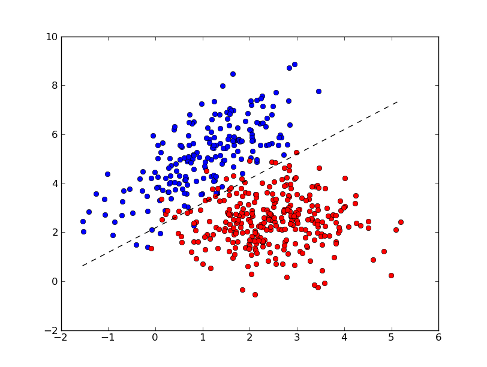
\includegraphics[width=8cm]{images/lda.png}
	\caption{Classification LDA}
	\label{classiLDA}
\end{figure}

\smallbreak
\textbf{Principes de LDA : }
\smallbreak

Le principe de la méthode LDA est illustré par les deux figures suivantes. Il a été supposé que deux observables , X et Y, étaient accessibles à l'observateur. Les zones bleues sont éliminées par les coupures (qui sont représentées par les lignes bleues).

Les deux premiers graphiques montrent le résultat de coupes classiques : on peut voir le compromis réalisé dans les deux cas entre précision et efficacité (Figure \ref{principeLDA1}).


\begin{figure}[h]
	\centering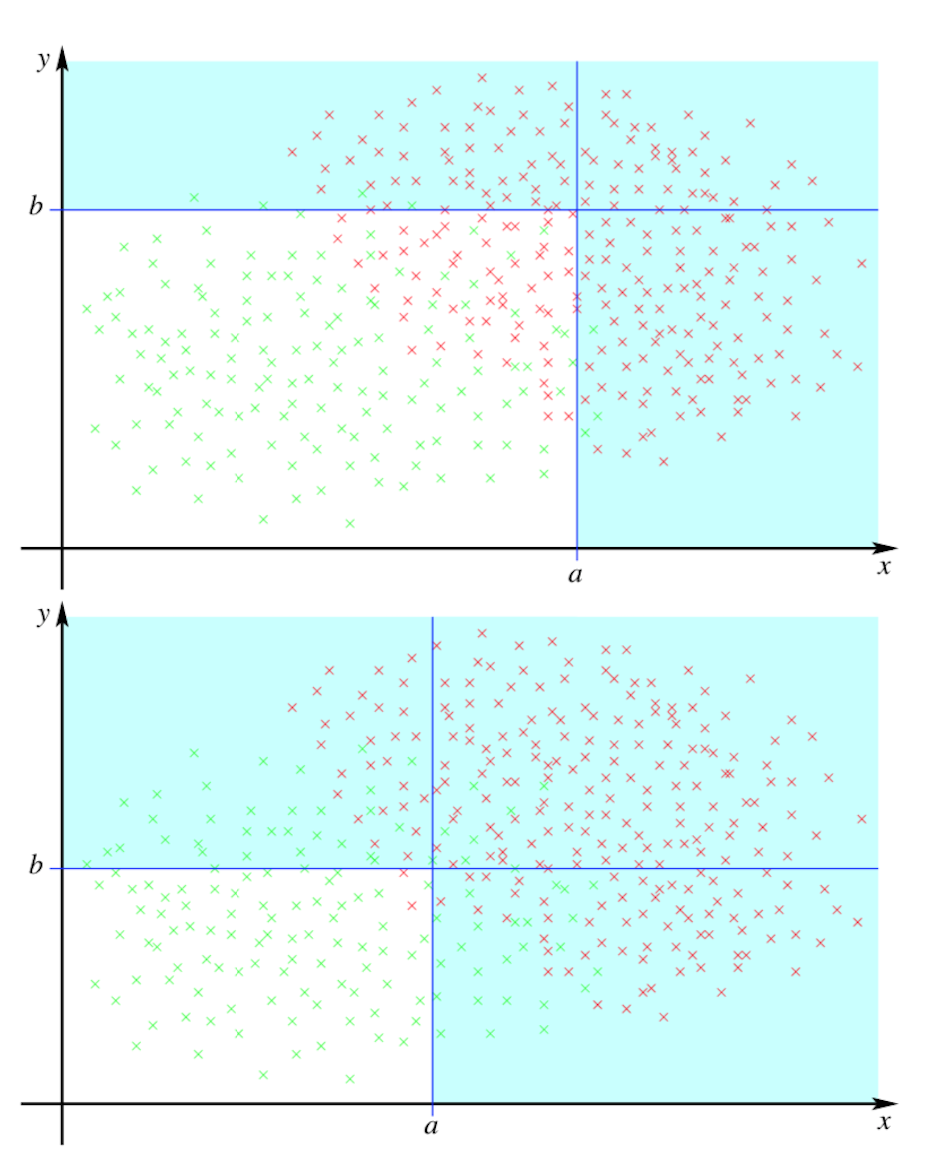
\includegraphics[width=8cm]{images/principeLDA1.png}
	\caption[Principe de LDA 1]{Principe de LDA 1 \cite{Faivre}}
	\label{principeLDA1}
\end{figure}

LDA consiste à découper le long d'une combinaison linéaire de tous les observables, plutôt que le long de chacun des observables. Cette combinaison linéaire est définie par une direction LDA (ou axe). 

L'algorithme consiste à calculer la direction de cet axe de manière à avoir une discrimination optimale entre les classes conformément à un critère donné. Un hyperplan perpendiculaire à l'axe est alors associé à cette discrimination (Figure \ref{principeLDA2}]).

\begin{figure}[h]
	\centering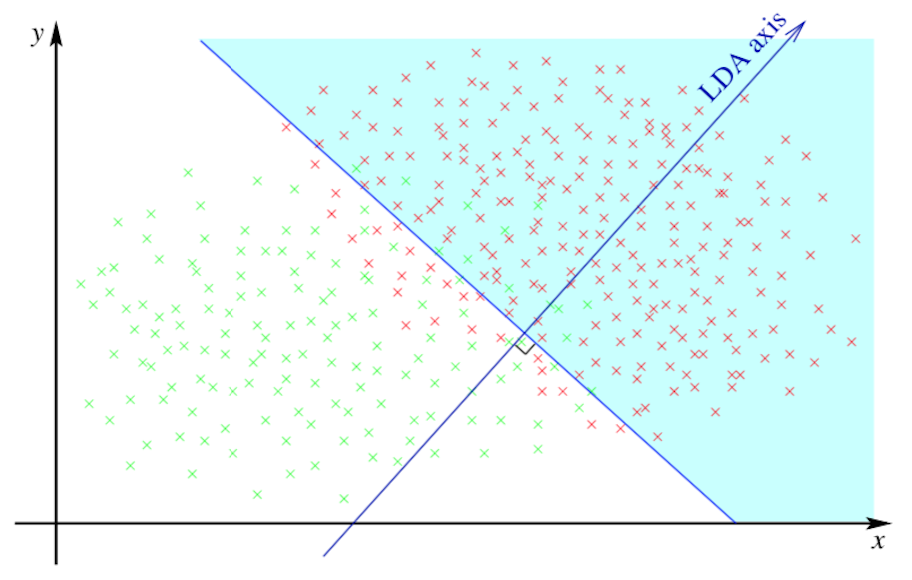
\includegraphics[width=8cm]{images/principeLDA2.png}
	\caption[Principe de LDA 2]{Principe de LDA 2 \cite{Faivre}}
	\label{principeLDA2}
\end{figure}

\textbf{Hypothèses et formules : }
\smallbreak

L’objectif est de produire une règle d’affectation $X(\omega) \mapsto Y(\omega)$ qui permet de prédire, pour une observation $\omega$ donnée, sa valeur associée de Y à partir des valeurs prises par X.

La règle bayesienne consiste à produire une estimation de la probabilité à posteriori (appuyée sur les expériences et les faits) d’affectation :

\begin{equation}
P(Y=y_k ~|~ X) = \frac{P(Y=y_k) \times P(X ~|~ Y=y_k)}{\sum_{i=1}^K P(Y=y_i) \times P(X ~|~ Y=y_i)}
\end{equation}

$P(Y=y_k)$ est la probabilité d’appartenance à une classe. $P(X ~|~ Y=y_k)$ représente la fonction de densité des X conditionnellement à la classe $y_k$.

La règle d’affectation pour un individu $\omega$ à classer devient alors :

\begin{equation}
Y(\omega) = \arg\max_{k}\ P(Y=y_k ~|~ X(\omega))
\end{equation}

Toute la problématique de l’analyse discriminante revient alors à proposer une estimation de la quantité :

\begin{equation}
P(X ~|~ Y = y_k)
\end{equation}

On distingue principalement deux approches pour estimer correctement la distribution $P(X ~|~ Y=y_k)$ :
\smallbreak
\begin{itemize}
	\item L’approche non-paramétrique n’effectue aucune hypothèse sur cette distribution mais propose une procédure d’estimation locale des probabilités, au voisinage de l’observation $\omega$, à classer. Les procédures les plus connues sont la méthode d'estimation par noyau et la méthode des plus proches voisins.
	\smallbreak
	\item La seconde approche effectue une hypothèse sur la distribution des nuages de points conditionnels, on parle dans ce cas d’analyse discriminante paramétrique. Exemple : hypothèse de multinormalité, etc.
	\smallbreak
\end{itemize}

\subsubsection{Support Vector Machine}
\label{subsubsection : 4.Support Vector Machine}
SVM est une méthode de classification binaire par apprentissage supervisé, destinée à résoudre des problèmes de discrimination (décider à quelle classe appartient un échantillon) et de régression (prédire la valeur numérique d'une variable). 

Cette méthode repose sur l'existence d’un classificateur linéaire dans un espace approprié. 

Puisque c’est un problème de classification à deux classes, cette méthode fait appel à un jeu de données d'apprentissage pour apprendre les paramètres du modèle. Elle est basée sur l'utilisation de fonction dites noyau qui permettent une séparation optimale des données. 

Après la méthode  LDA, c'est la deuxième méthode la plus populaire parmi les classificateurs linéaires.

\subsubsection{Bayes quadratique}
\label{subsubsection : 4.Bayes Quadratique}
Cette approche est basée sur le calcul de la probabilité de chaque classe, compte tenu du vecteur de caractéristiques. Bayes quadratique assigne le signal EEG à la classe la plus probable. Ce classificateur nest pas très populaire pour les systèmes BCI, cependant , il reste assez précis pour la classification de l'imagerie motrice (motor imagery) comparé à d'autres méthodes.

Nous avons décidé de partir sur l'algorithme LDA car nous souhaitons travailler en temps réel, et il se trouve que la méthode LDA  semble être la plus performante pour ce genre de tâche.


%Bibliographie : 

% Site web de McGill : http://lecerveau.mcgill.ca/flash/i/i_01/i_01_cr/i_01_cr_ana/i_01_cr_ana.html#2    

% Livre EEG Signal Processing 

% Mémoire de Olivier St-Amand " Techniques de traitement de signal appliquées aux essais individuels évoqués

%SSVEP A Survey of Stimulation Methods Used in SSVEP-Based BCIs